\section{Specific requirements}
\label{sec:specreq}

  \subsection{External interface requirements}

    \subsubsection{User interfaces}
    \label{sec:userinterfaces}

\begin{figure}[h!]
      \centering

      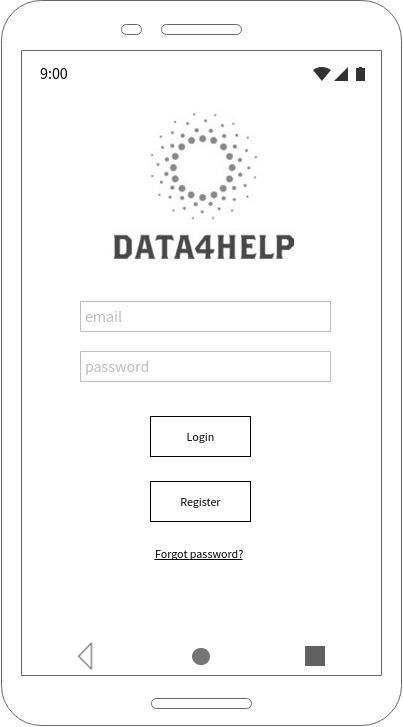
\includegraphics[width=0.25\textwidth]{img/mockup/homepage.jpg}

  \caption{Homepage}

\end{figure}

%\clearpage

\begin{figure}[h!]
  \centering

  \begin{subfigure}[b]{0.25\linewidth}

    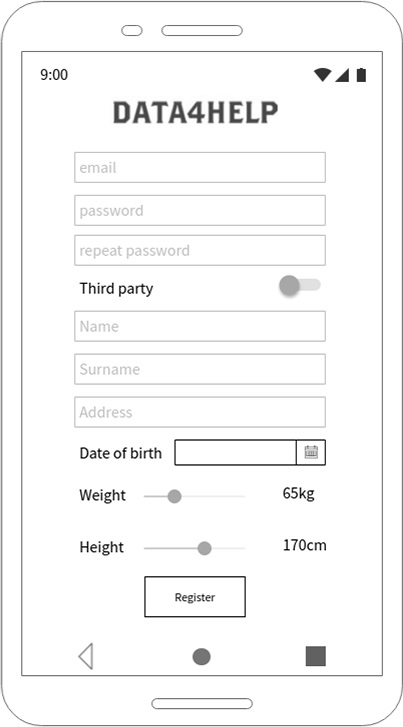
\includegraphics[width=\linewidth]{img/mockup/u_registration.jpg}

    \caption{User Registration}

  \end{subfigure}
 ~ ~ ~ ~ ~ ~
  \begin{subfigure}[b]{0.25\linewidth}

    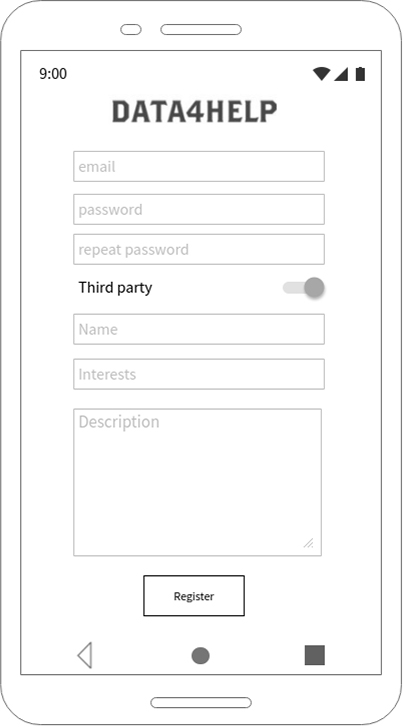
\includegraphics[width=\linewidth]{img/mockup/tp_registration.jpg}

    \caption{Third Party Registration}

  \end{subfigure}

\caption{Registration Form}

\end{figure}

\clearpage

\begin{figure}[h!]

 \centering

  \begin{subfigure}[b]{0.25\linewidth}

    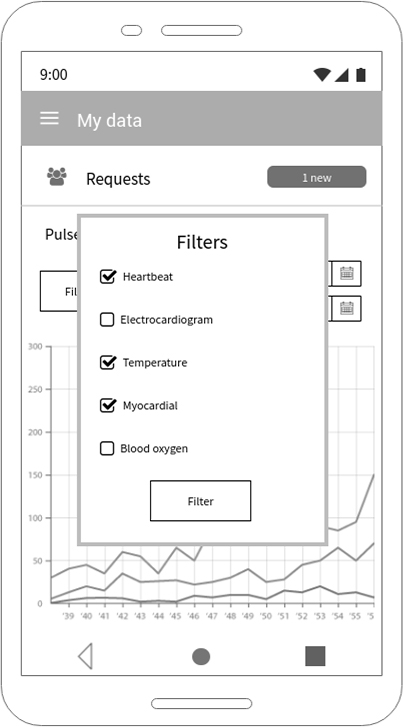
\includegraphics[width=\linewidth]{img/mockup/u_filters.jpg}

    \caption{User Filters}

  \end{subfigure}
 ~ ~ ~ ~ ~ ~ 
  \begin{subfigure}[b]{0.25\linewidth}

    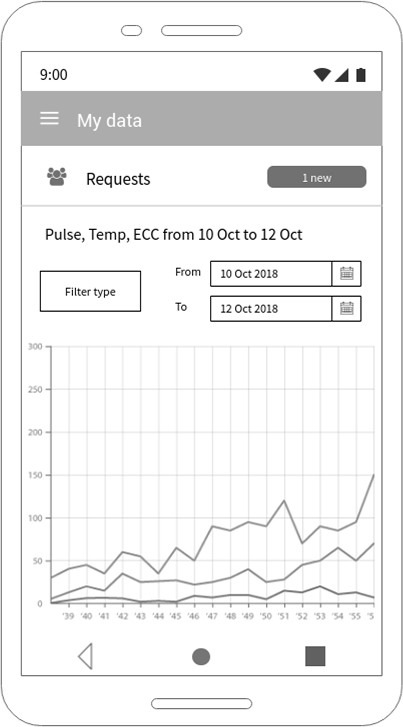
\includegraphics[width=\linewidth]{img/mockup/u_data.jpg}

    \caption{User Data}

  \end{subfigure}

\caption{Interface for Graphical representation of User Data }

 \end{figure}

%\clearpage

\begin{figure}[h!]

 \centering

  \begin{subfigure}[b]{0.25\linewidth}

    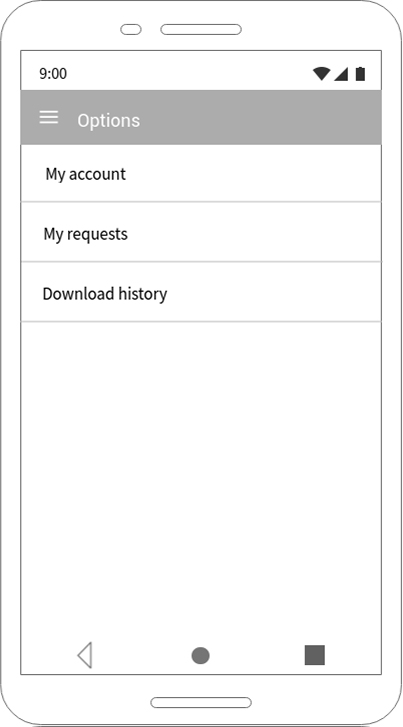
\includegraphics[width=\linewidth]{img/mockup/tp_options.jpg}

    \caption{Third Party Options}

  \end{subfigure}
 ~ ~ ~ ~ ~ ~ 
  \begin{subfigure}[b]{0.25\linewidth}

    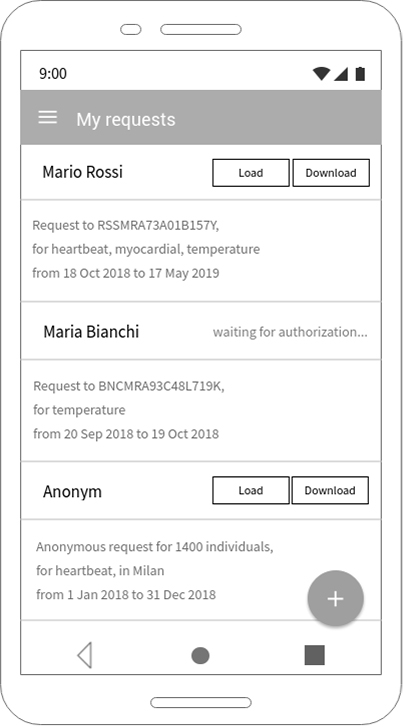
\includegraphics[width=\linewidth]{img/mockup/tp_requests.jpg}

    \caption{Third Party Requests}

  \end{subfigure}

\caption{Third Party management of Account }

 \end{figure}

\clearpage

\begin{figure}[h!]

 \centering

  \begin{subfigure}[b]{0.25\linewidth}

    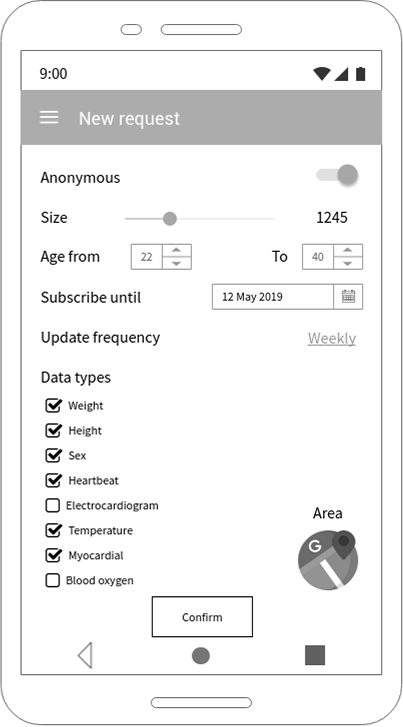
\includegraphics[width=\linewidth]{img/mockup/tp_areq.jpg}

    \caption{Anonymous-Group Request}

  \end{subfigure}
 ~ ~ ~ ~ ~ ~ 
  \begin{subfigure}[b]{0.25\linewidth}

    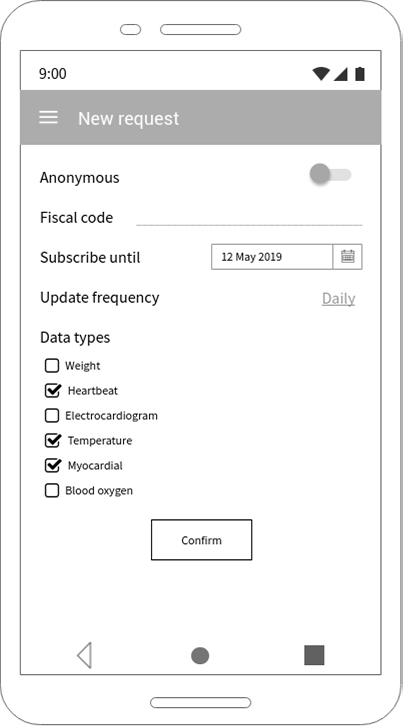
\includegraphics[width=\linewidth]{img/mockup/tp_sreq.jpg}

    \caption{Single-User Request}

  \end{subfigure}

\caption{Third Party management of Account }

 \end{figure}

%\clearpage

\begin{figure}[h!]

 \centering

  \begin{subfigure}[b]{0.25\linewidth}

    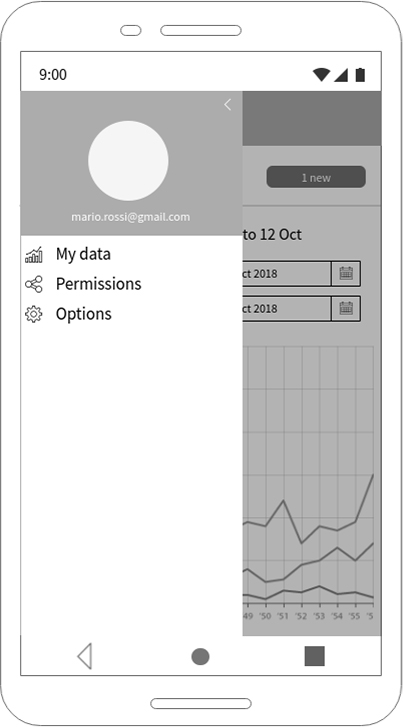
\includegraphics[width=\linewidth]{img/mockup/u_sidebar.jpg}

    \caption{User Sidebar}

  \end{subfigure}
 ~ ~ ~ ~ ~ ~ 
  \begin{subfigure}[b]{0.25\linewidth}

    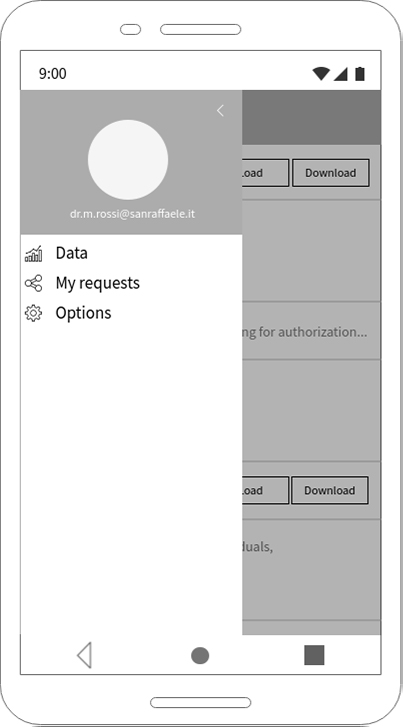
\includegraphics[width=\linewidth]{img/mockup/tp_sidebar.jpg}

    \caption{Third Party Sidebar}

  \end{subfigure}

\caption{Sidebar}

 \end{figure}

\clearpage

\begin{figure}[h!]

 \centering

   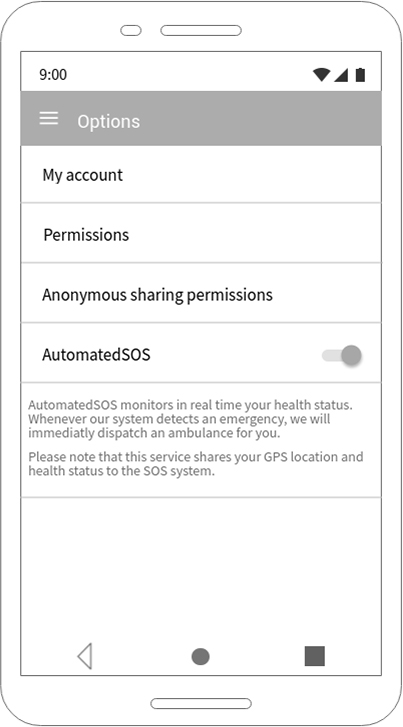
\includegraphics[width=0.25\textwidth]{img/mockup/u_options.jpg}

    \caption{User Options}

\end{figure}

%\clearpage

\begin{figure}[h!]

 \centering

  \begin{subfigure}[b]{0.25\linewidth}

    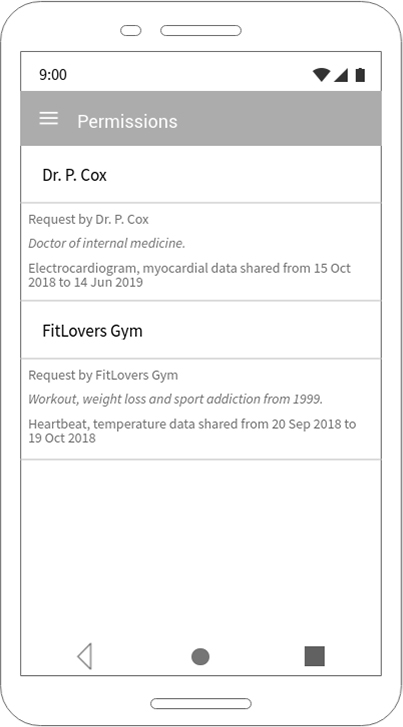
\includegraphics[width=\linewidth]{img/mockup/u_permissions.jpg}

    \caption{List of all Third Party that has access to User Data}

  \end{subfigure}
 ~ ~ ~ ~ ~ ~ 
  \begin{subfigure}[b]{0.25\linewidth}

    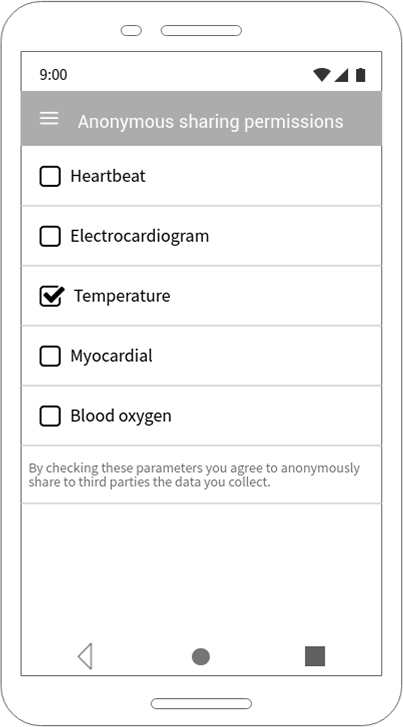
\includegraphics[width=\linewidth]{img/mockup/u_anonym.jpg}

    \caption{User Data that can be shared with Third Parties}

  \end{subfigure}

  \caption{Anonymous User Data Sharing Management}

 \end{figure}

\clearpage

\begin{figure}[h!]

 \centering

  \begin{subfigure}[b]{0.25\linewidth}

    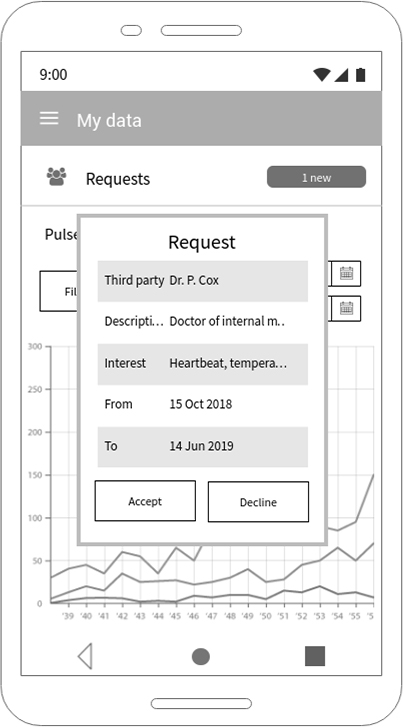
\includegraphics[width=\linewidth]{img/mockup/u_request.jpg}

    \caption{User request to share single Data}

  \end{subfigure}
 ~ ~ ~ ~ ~ ~ 
  \begin{subfigure}[b]{0.25\linewidth}

    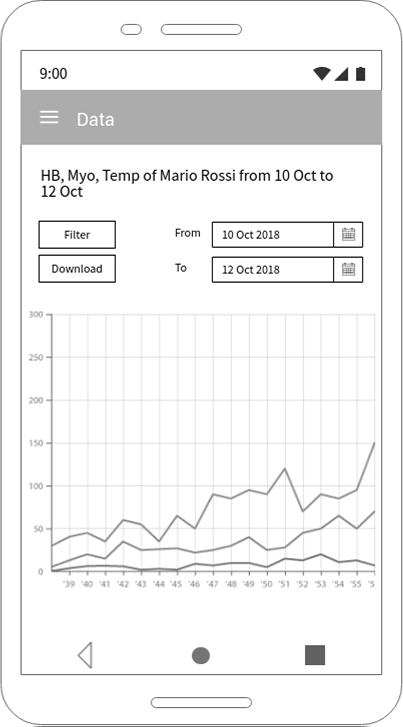
\includegraphics[width=\linewidth]{img/mockup/tp_data.jpg}

    \caption{Single-User Data shared}

  \end{subfigure}

  \caption{Single-User Data  Management}

 \end{figure}

\clearpage

    \subsubsection{Hardware interfaces}

The area in which the system operates is Data Management hence no hardware interfaces has to be implemented. Indeed a software-based product is enough to perform these functions.

    \subsubsection{Software interfaces}

    \subsubsection{Communication interfaces}

  \subsection{Functional requirements}

    \begin{description}
      \item[Account handling]
      \item[\texttt{R.A1}] The system shall allow users registration
      \item[\texttt{R.A2}] The system shall allow third party registration
      \item[\texttt{R.A3}] The system shall distinguish between user and third party accounts
      \item[\texttt{R.A4}] The system shall guardantee account uniqueness by not allowing two account to have the same email
      \item[\texttt{R.A6}] The system shall allow users and third parties to access their account (\textit{login}) only if they provide correct email and password
      \item[\texttt{R.A7}] The system shall allow users and third parties to exploit \texttt{Data4Help} and \texttt{AutomatedSOS} functionalities only if they are \textit{logged in} their account

      \item[Data encoding]
      \item[\texttt{R.D1}] The system shall encode data received through wearables'sensors and store it internally\footnote{for example the system can store data into an internal database or can save it using a cloud service; the important aspect is that data must be retrivable in the future}
      \item[\texttt{R.D2}] The system shall be able to retrive data previously stored on request
      \item[\texttt{R.D3}] The system shall not erase data once it is stored internally
      \item[\texttt{R.D4}] Once the system stored data, it shall allow access to that data only to the user account that was \textit{logged in} while the data was collected
      \item[\texttt{R.D5}] The system shall be able to share the stored data to more than one account
      \item[\texttt{R.D6}] The system shall be able to compose groups of data entries (\textit{aggregate data}) and anonymize them (every data entry in the group has no information about the providing user, such as fiscal code or email)

      \item[Interfaces]
      \item[\texttt{R.I1}] The system shall provide a registration form for users and third parties
      %TODO in case there are no data? Interface will not render anything: the requirement says that the interface shall be ABLE to render data in enery case, so I think it's fine
      \item[\texttt{R.I2}] The system shall provide to the user an interface able to render data graphically, allowing filters like time interval or data type
      \item[\texttt{R.I3}] The system shall provide a request form to the third parties

      \item[Data sharing requests]
      \item[\texttt{R.R1}] The system shall allow third parties to ask for data sharing of a single user
      \item[\texttt{R.R2}] The system shall ask the user to accept or decline every single-user request of data sharing by third parties that has him/her as target user
      \item[\texttt{R.R3}] The system shall provide access to the target user data to the third party only if the user accepted the request of the third party, otherwise the system shall notify to the third party that the user declined the request
      \item[\texttt{R.R4}] The system shall allow third parties to ask for data sharing of \textit{aggregate data}
      \item[\texttt{R.R5}] The system shall be able to check if a request for \textit{aggregate data} by a third party can be properly anonymized (there shall be at least 1000 user data entries that fit the parameters of the request)
      \item[\texttt{R.R6}] The system shall provide access to the \textit{aggregate data} to the third party only if the the request can be properly anonymized, otherwise the system shall notify the third party that its request cannot be properly anonymized
      \item[\texttt{R.R7}] The system shall provide access to a third party to newly produced data if it fits the third party request
      % TODO add refernce to the request structure, because this requirement is a bit ambiguous

      \item[SOS calls]
      \item[\texttt{R.S1}] The system shall provide to the user an option to apply to \texttt{AutomatedSOS}
      \item[\texttt{R.S2}] If user applied to \texttt{AutomatedSOS}, the system shall monitor his/her parameters in real time by checking whether they are above or below the thresholds
      % TODO add reference
      \item[\texttt{R.S3}] If user applied to \texttt{AutomatedSOS} and his/her health parameters are critical (above or below thresholds), the system shall send an emergency call to the SOS system
      \item[\texttt{R.S4}] When the system sends an emergency call, it shall provide to the SOS system API user's GPS location and user's health status through his/her critical parameters encoding

    \end{description}

  \subsection{Scenarios}

\subsubsection{Scenario on Stroke detection} % FABIO ho fatto alcune correzioni allo scenario 1. Visto che è la parte della quale ti sei occupato tu, preferisco non procedere e chiederti prima se ti vanno bene; ho cambiato qualcosina nel testo e corretto un paio di sviste grammaticali
    \label{sec:}

      Luke is a 65 years old man that after 40 years of work at the post office finally got retired. Because of the sedentary nature of his work he is worried that he may suffer a stroke.

      In order to monitor his health parameters, % FABIO tolto last week; cambiato today in "after some days" per rimanere generico
      he downloads the \texttt{Data4Help} app. The system allows him to create an account after filling all the required information(see Table~\ref{tab:login}). The system explicitly asks Luke if he wants to join the \texttt{AutomatedSOS} service and Luke accepts sharing his heartbeat and myocardial with the app.

The system will now on check in real time Luke's health parameters that will be collected through his smartwatch. % FABIO potremmo aggiungere che ha un braccialetto col battito cardiaco, altrimenti non si capisce bene come faccia il sistema a rilevare i suoi parametri

      After some days Luke's health parameters exceede thresholds because of a stroke: the system recognizes immediatly the critical situation and forwards in less than 5 seconds an emergency notification to SOS system, providing the Luke's GPS location and health status feedback.


    \subsubsection{Scenario on Anonymous-Group Request}

    The franchise BodySlim is opening a new gym in Milan near Parco Sempione;the most relevant aspect that characterize it, is the timetable:open 365 days, 8 hours per day. 

In order to maximize the revenue the management would like to know in which time of the day the potential customers make exercise.\\A reliable sample can be obtained from Data4Help, therefore BodySlim create a third party account filling all the required third party information (see Table 1). 

Then the franchise make an anonymous-group request (see Table 2) for 2000 individuals with particular characteristics: age between 20 and 60,at least once a week they are running in Parco Sempione(this can be checked with GPS position) to Data4Help. 

The app find in his internal database these 2000 users and therefore the system immediately shares the required information with BodySlim without asking to the users the authorization .

Now looking at the most common hours chosen for running by these individuals the manager can easily identify the most profitable hours in which the gym should be opened.

    %Otherwise if the research is not successfully, Data4Help denied the request of BodySlim which has to find another way to obtain a reliable sample.
    %NO ALTERNATIVES:THIS IS AN EXAMPLE/AN APPLICATION

    \subsubsection{Scenario on Single-User Request}

    Rose has just discovered that is expecting a daughter. Harold, her gynecologist, needs to keep monitoring bloody ossygen,electrocardiogram and pulse in order to understand if the pregnancy is proceeding well or not. 

Therefore he creates a third party account of Data4Help and after the system has checked if the required information(see Table 1) has been correctly inserted, he requires these data to the app. 

According to the single-user request(see Table 2)  policy Data4Help asks to Rose the consensus for sharing these data. Rose,which really care about her daughter's health, immediately gave the authorization to the app that can make them available to her gynecologist.

 Nine months later the beautiful and healthy Marie is born.
    %her motherRose which is worried about her privacy, wouldn't like to share his personal data anymore so decides to unsubscribe to Data4Help. The system after having received the request, delete her Dataset and her account. From now on neither the gynecologist nor Data4Help will be able to access to Rose's data.

    \subsubsection{Scenario on subsribing to new data}

    Jack is a policeman that has decided to spend his holidays in a spa called "BeautySPA" which allow him to loss 15 kg thanks to fitness activity and a healthy diet.In order to understand if this treatment is efficient over time the spa and Jack decides that user's health parameters like height,weight and body temperature must be monitored. 

Therefore the policeman and BeautySPA create respectively a user and a third party account of Data4Help and the system ,after checking that all the required information (see Table 1)are properly added, allow them to exploit all Data4Help functionalities.

 Indeed  BeautySPA immediately apply for the three Jack's health parameters to the app. 

The app recognize this as a single-user request(see Table 2)  so asks to Jack the authorization whether to provide them to the spa or not. 

Obviously he accept and therefore Data4Help make available these data. 

Unfortunately after just 1 month the policeman has already had a weight increase of 6 kg. So in order to better understand which may be the reasons the spa asks more health parameters such as blood oxygen and heartbeat to Data4Help which again,before sharing these data with BeautySPA, will ask the authorization of the user.

     \subsubsection{Scenario on Graphical Interface}
     Paul is studying Telecommunication Engineering at Politecnico di Milano and would like to partecipate at the PolimiRun therefore he is training twice a week since January(the PolimiRun occurs in May).

 The telecommunication student decides to create a User Account sharing heartbeat and blody ossygen with Data4Help. 

The system checks that all the required information are properly added then it starts to periodically collect the two user data entries creating a Dataset for the student. 
%ALBERTO controlla se ti convincono data entry,dataset usate cosi

At the end of April Paul is worried that despite all the efforts the PoliRun is beyond his physical capacities so he resolves to unsubsribe to that competition but then remember that Data4Help lets the users to see in a personalized way all the data collected provided that they are logged in their account. 

Consequently Paul,after the login in, asked to the app to show his blody ossygen and heartbeat from January to April. 

The system retrieves the required data and make them available to the student through the graphical interface of the app.

 In this way Paul can see the evolution of these two health parameters during the four months and immediately understands that the PolimiRun is absolutely realistic for him thanks to an impressive improvement in the concentation of blody ossygen and a reduction of heartbeat per minute.

    \subsubsection{Anonymous Group Request}
%ALBERTO controlla se ti torna usare la posizione GPS in questo modo
    FastAndEasy, a car-sharing company, has a business model based on how much time his users rent one of his car in a week. After 5 years the society has to decide whether change this model with a new one based on the kilometers travelled in a week or keep going with the old one. 

In order to take the right decision FastAndEasy needs to know the GPS location of all of his users when they are driving his cars(so not 24 hours a day) for 3 months.

 Because of this is a temporary solution it will be a waste of money for the car-sharing company to implement his own system for picking up these data. Therefore FastAndEasy creates a third party account of Data4Help filling all the required third party information (see Table 1) and asks to the app to provide the GPS location only of his users(which can be identified by the fiscal code).

This is a Single-user(Table 2) request therefore  Data4Help will ask directly to the specified users whether accept or deny it.

 Indeed only for the users who accept the request the app will grant the access to their GPS location to the company which,  looking at the data collected after 3 months, can compute the possible earnings of the new model,compare them with the old ones and finally make a decision.



  \subsection{Use cases}


% FABIO diamo un nome specifico agli use cases e agli scenari?
%ALBERTO Per gli use cases è già nella tabella 3 e in ogni use case c'è già il campo  nome

      \begin{table}[h!]
        \centering
        \begin{tabularx}{\linewidth}{|c|X|}
          \hline

          \textbf{Name} & Sign in of User in Data4Help\\
        	\hline

        	\textbf{Actors} & User \\
        	\hline

        	\textbf{Entry Condition} & Data4Help is downloaded on the smartphone \\
        	\hline

        	\textbf{Flow of Events} & 1.User click on "Create a new User account" button in the homepage of the app.

        					2.User fills all the mandatory fields("Age", "Name", "Surname", "Email", "Sex", "Password", "Fiscal 							Code").

        					3.User insert in the fields "Shared Data" the data that he want to share with the app.

        					4.User clicks on the "Confirm" button.

        					5.The system create a DataSet for the User in his internal database.\\
        	\hline

        	\textbf{Exit Condition} & The User account has been successfully created. \\
        	\hline

        	\textbf{Exceptions} &
        					%1. The system find that User filled the field "Age" with 12.
        					1.The system finds that User filled the field "Email"  with an email that is non-existent or that has 							already been associated with another user.

        					2.The system finds that User filled the field "Fiscal Code" with an expression not long 16 								characters.

        					3.The system finds that User filled the field "Password" with an expression shorter than 8 								characters.

        					All exceptions are handled notifying the issue to the User and taking back the \textbf{Flow of 							Events} to the point 2.\\
          \hline
        \end{tabularx}
      \end{table}

      \begin{table}[h!]
        \centering
        \begin{tabularx}{\linewidth}{|c|X|}
          \hline

          \textbf{Name} & Log in of User \\
        	\hline

        	\textbf{Actors} & User \\
        	\hline

        	\textbf{Entry Condition} & User has already created an account\\
        	\hline

        	\textbf{Flow of Events} & 1.User opens the app on his smartphone.

        					2.User insert his email in the field "Email" in the homepage of Data4Help.

        					3.User insert his password in the field "Password" in the homepage of Data4Help.

        					4.User Click on "Log In" button in the homepage of the app.\\
        	\hline

        	\textbf{Exit Condition} & User is successfully Logged in and can exploit all the functionalities of the app. \\
        	\hline

        	\textbf{Exceptions} & 1.The system doesn't find the email address inserted in the field "Email" in his internal DataBase.

        				In this case the \textbf{Flow of Events} has to be executed again from step 2.

        				2.The system doesn't find the password inserted in the field "Password" in his internal DataBase.

        				 In this case the \textbf{Flow of Events} has to be executed again from step 3.

        				3.The system find both the email and the password inserted by User but these refers to 2 different users.

        				In this case the \textbf{Flow of Events} has to be executed again from step 2. \\
          \hline
        \end{tabularx}
      \end{table}



      \begin{table}[h!]
        \centering
        \begin{tabularx}{\linewidth}{|c|X|}
          \hline

          \textbf{Name} & Accept Single-User request\\
        	\hline

        	\textbf{Actors} & Third party and User \\
        	\hline

        	\textbf{Entry Condition} & Third party and User have already created respectively a third party and a user account and they 							are already logged in in Data4Help.\\
        	\hline

        	\textbf{Flow of Events} & 1.Third party clicks on the button "Single-User Request".

        					2.Third party inserts the Fiscal Code of the User in the field "Fiscal Code" of the Single-User 								Request page.

        					3.Third party lists to the system the data of the User which it would like to access filling the field 							"DataRequired" in the Single-User Request page.

        					4.The system asks to the User whether he accepts or denies to share those specified data with the 					Third party.

        					5.User answers clicking in the field "Yes" in his homepage.

        					6.The system make available the data for the third party.\\
        	\hline

        	\textbf{Exit Condition} & Third party can exploit the data \\
        	\hline

        	\textbf{Exceptions} & 1.The system doesn't find the fiscal code inserted by third party in the field "Field Code" in his internal 				database.

        				In this case the \textbf{Flow of Events} has to be executed again from step 2.

        				2.The system discovers that the User has denied the request therefore Data4Help notifies this 							information to the third party which won't have access to the required data.

        				The third party can 	make a new Single-User request referred to a new User: in this case the 							\textbf{Flow of Events} has to executed again from the first step.\\

          \hline
        \end{tabularx}
      \end{table}


      \begin{table}[h!]
        \centering
        \begin{tabularx}{\linewidth}{|c|X|}
          \hline

          \textbf{Name} & Call an ambulance\\
        	\hline

        	\textbf{Actors} & User and SOS System\\
        	\hline

        	\textbf{Entry Condition} & User has actived AutomatedSOS and his health parameters exceedes thresholds\\
        	\hline

        	\textbf{Flow of Events} & 1.The system collects GPS location and health status parameters of the User from his internal 						database.

        					2.The system makes an emergency call to SOS System by providing GPS location and health 							status feedback of the User.

        					3.The SOS System accepts the call and dispatches the ambulance to the User location.

        					4.The SOS System notifies the system when the ambulance arrives at User Location.\\
        	\hline

        	\textbf{Exit Condition} & The ambulance is taking care of the User. \\
        	\hline

        	\textbf{Exceptions} & \\
        	\hline

        	\textbf{Special Requirements} & 1.The system has to collect the GPS location,health parameters of the User and make the 							emergency call to SOS System within five seconds from the time the health parameters 							exceedes thresholds.\\
          \hline
        \end{tabularx}
      \end{table}

   

      \begin{table}[h!]
        \centering
        \begin{tabularx}{\linewidth}{|c|X|}
          \hline

          \textbf{Name} & Accept Anonymous-Group request\\
        	\hline

        	\textbf{Actors} & Third Party\\
        	\hline

        	\textbf{Entry Condition} & Third party has already created a third party account and is already logged in in Data4Help.\\
        	\hline

        	\textbf{Flow of Events} &
        					1.Third party clicks on the button "Anonymous-Group Request".

        					2.Third party lists to the system which data requires filling the field "Data Required" in the 							Anonymous-Group request page.

        					3.The system looks for, in his internal database, the User's Datasets  which fit with the request 						made by the third party.

        					4.The system aggregate the data found and anonymize them.

        					5.The system provides the anonymous data to the third party.\\
        	\hline

        	\textbf{Exit Condition} & Third party can exploit the data \\

        	\hline

        	\textbf{Exceptions} & 1.The data cannot be anonymized  by the system because it doesn't find at least 1000 							User Datasets which match with the third party request. Therefore the system cannot 							grant access to the data to the third party and has to notify her this information .

        						The third party can make a new Anonymous-Group request asking for a new set of data: 							in this case the \textbf{Flow of Events} has to be executed again from the first step.\\

          \hline
        \end{tabularx}
      \end{table}





      \begin{table}[h!]
        \centering
        \begin{tabularx}{\linewidth}{|c|X|}
          \hline

          \textbf{Name} & Show Data previously acquired\\
        	\hline

        	\textbf{Actors} & User\\
        	\hline

        	\textbf{Entry Condition} & User has already created a User account and is already logged in in Data4Help.\\
        	\hline

        	\textbf{Flow of Events} &
        					1.User clicks on the button "Data Management".

        					2.User decides which filter has to be applied to his DataSet filling the field "Filters" in the Data 						Management page.

        					3.The system organize the User's DataSet following the User's instructions.

        					4.The system show to the User these data thanks to a graphical interface. \\
        	\hline

        	\textbf{Exit Condition} & User can see his data in the specified way\\

        	\hline

        	\textbf{Exceptions} & 1 The system hasn't gathered any data yet because the user has just created an account.

        				Thanks to the graphical interface the system notifies the user that no data can be shown.

        				Only after having collected some data the User can specified filters:the \textbf{Flow of Events} must be 				executed from the first step.\\

          \hline

        \end{tabularx}
      \end{table}

   

      \begin{table}[h!]
        \centering
        \begin{tabularx}{\linewidth}{|X|X|}
          %|X| let to go in a new line on a cell
          \hline

          \textbf{Use Case ID} & \textbf{Name}  \\
        	\hline

        	1 & Sign in of User in Data4Help\\
        	\hline

        	2 & Log in of User\\
        	\hline

        	3 & Accept Single-User request\\
        	\hline

        	4 & Call an Ambulance\\
        	\hline

        	5 & Accept Anonymous-Group request\\
        	\hline

        	6 & Show Data Previously Acquired\\
          \hline

  	    \end{tabularx}
        \caption{Traceability Matrix}
      \end{table}

  

      \begin{table}[h!]
        \centering
        \begin{tabularx}{\linewidth}{|X|X|X|X|}
          %|X| let to go in a new line on a cell
          \hline
          \textbf{Raw ID} & \textbf{Goal ID} & \textbf{Req ID} & \textbf{Use Case ID} \\
          \hline

	        r1 & \texttt{G.U.1} & \texttt{R.A1}  \newline \texttt{R.A3}  \newline \texttt{R.A4} \newline \texttt{R.I.2}& \texttt{1} \\
          \hline

	        r2 & \texttt{G.U.1} & \texttt{R.A3}  \newline \texttt{R.A6}  \newline \texttt{R.A7} & \texttt{2}  \\
	\hline

	        r3 & \texttt{G.T.1} & \texttt{R.A3}  \newline \texttt{R.I.3}  \newline \texttt{R.R.1} \newline \texttt{R.R.2} \newline \texttt{R.R.3}& \texttt{3}  \\
          \hline

          r4 & \texttt{G.U2} & \texttt{R.S1} \newline  \texttt{R.S2} \newline \texttt{R.S3}\newline \texttt{R.S4} & \texttt{4}   \\
          \hline

          r5 & \texttt{G.T2} & \texttt{R.A3} \newline  \texttt{R.D2} \newline \texttt{R.D5}\newline \texttt{R.D6}  \newline \texttt{R.I.3} \newline \texttt{R.R4}  \newline \texttt{R.R5}  \newline \texttt{R.R6} & \texttt{5}   \\
          \hline

          r6 & \texttt{G.U1} & \texttt{R.A3} \newline \texttt{R.A7} \newline  \texttt{R.I2} \newline  \texttt{R.D2} & \texttt{6}   \\
          \hline

      \end{tabularx}
      \end{table}
%everything referred to the system

  \subsection{Performance requirements}
  \label{sec:performance}

    \textbf{AutomatedSOS} implements a very important function:monitoring the human health; in this field having a lower time response can save a life.

    Therefore, when the system detects than at least one of the health parameters exceedes the thresholds (user is in health danger),it must collect all the required data(GPS location and user's health status) and send them through an emergency call to an external service(SOS System) within 5 seconds.

    Moreover Data4Help has to send every 1 second the required data to the subscribed third parties(both for Single-User requests and for Anonymous-Group requests) in order to grant them accurate enough data.

    \texttt{AutomatedSOS} time performances are critical: the emergency call must be delivered no more than 5 seconds after the health danger detection, in order to have an ambulance dispatched from the SOS system as soon as possible. It is important to note again that \texttt{AutomatedSOS} is in charge only of the emergency call.

  \subsection{Design constraints}
    \subsubsection{Standards compliance}
%TODO decidere se già descitto in 2.4.3

    \subsubsection{Hardware limitations}
The smartphone, in which the app(both for User account and Third Party Account) is downloaded, must guarantee that all the system functionalities can be correctly performed; hence the only compatible smartphones are the ones with : iOS or Android as operating system,3G/4G connection and can retrieve GPS location.

 Moreover is necessary that each user has his own physical device and this device must be able to collect all the data that the user decides to share with the app otherwise the system won't be able to perform the Data Gathering function(\ref{sec:datagathering}).

    \subsubsection{Any other constraint}
%TODO Superfluo?
  \subsection{Software system attributes}

    \subsubsection{Reliability}
      The sofware is expected to work continuously for 24 hours a day despite small deviations are accepted. 

      Moreover as section 3.6.4 says, the sofware changes during time, so each time the software is modified is necessary to check the consequences on the reliability.

    \subsubsection{Availability}

      The system is expected to be available for 99.99 \% of the time but in case of failure it must be able to recover within 1 second otherwise in case of user's health problem AutomatedSOS won't respect the constraint descibed in \ref{sec:performance} and therefore the user will be in a critical situation.

 There 2 different situations which may result in a failure:failed components or due to unexecpected increasing in the requests. 

At this level of abstraction is not strickly required but in both of these cases a distributed architecture is an optimal solution:indeed in case of failure one of the redundant component can replace the one offline and in case of high demand a load balancing between redundant component can minimize the probability of failure of the system.

    \subsubsection{Security}

      The system requires the users(both Data4Help and AutomatedSOS) and third Parties(only in Data4Help), in order to exploit all the functionalities of the app and avoid unauthorized access, to authenticate through email and password.

 These 2 credentials and all the Data collected by the system has to be securely stored in the internal database.

 Moreover as  requirement \texttt{R.D6} says for privacy issues for all the Anonymous-Group requests the system must not allow the third parties to link data collected to the users that produced them.
      %payment?

    \subsubsection{Maintainability}

      Data4Help, as \ref{sec:datagathering} says, has to collect data through multiple physical wearables devices therefore Data type handling should be implemented by the system in a flexible and extensible way, because wearables technologies change rapidly and our software should adapt in the least invasive way possible.

    \subsubsection{Portability}

      The system has to gather user's data through multiple devices as \ref{sec:datagathering} says. Therefore, must be guarantee that different physical wearables can easily send data to this product function for example thanks to some form of abstraction.

 In this way I will also have a significant cost reduction and an improvement in maintainability of the system.







